\documentclass[16pt,answers]{exam}
\author{Nima Poshtiban}
\title{Assignments of Arithmetic}
\usepackage{datetime}
\usepackage{amsmath}
\usepackage[utf8]{inputenc}
\usepackage{hyperref}
\usepackage{color}
\usepackage{graphics}
\newdate{date}{{26}{10}{2025}}
\date{\displaydate{date}}
\usepackage{float}

\begin{document}
	\maketitle
	\tableofcontents
	\pagebreak
	\section{Assignment No.1}
\paragraph{}
\textbf{Unconventional radices}
\begin{questions}
\question Convert the negabinary number $\mathbf{(0001 1111 0010 1101)_{-two}}$ to radix 16
	(hexadecimal).\label{a}
	\begin{solution}[space]
		From the Radix we can elicit the base logic for solving this problem\newline
		\begin{enumerate}
			\item Assuming the initial index is 1, Odd digits represents positive values whereas even digits are the quite opposite.
			\item Applying the deduction, a mathematical formula has been extracted from the logic:
			\[
			  0001 1111 0010 1101 \Longrightarrow \sum_{i=1}^{16}{(d_{i})\times2^{i-1}\times(-1)^{i} }
			\]
			\item Calculating the initial value:
			\(-2^{0} + -2^{2} + -2^{3} + -2^{5}  + - 2^{8}  + -2^{9} + -2^{10} + -2^{11} + -2^{12} \Longrightarrow 2781_{decimal}\)
			\item Conversion from \(radix=10\) to \(radix=16\)
			doing the chain division and residue operations the result is \( ADD_{radix=16} \)
		\end{enumerate}
	\end{solution}
\question Repeat part \ref{a} for radix $\mathbf{-16}$ (negahexadecimal).
	\begin{solution}[space]
	using the general conversion formula
	\[N=\sum_{i=0}^{n}{a_{i}(radix)^{i}}\]
	Step 1. from the privious solotion the \textbf{radix=10} value is \textbf{2781}, Applying the conversion
	\[
		\Longrightarrow \frac{2781}{-16} \Rightarrow q=-173\,,r=-3+16 = D
	\]
	Step 2. continue until quotient=0
	\[
		\Longrightarrow \frac{-173}{-16} \Rightarrow q=11\,r=-13+16 = 3  
	\]
	\[
		\Longrightarrow \frac{11}{-16} \Rightarrow q=0\,,r= -5 + 16 = B
	\]
	Step 3. put the numbers back together by LSF convention
	\[
		\Rightarrow B3D_{-16}
	\]
\end{solution}
\question Derive a procedure for converting numbers from radix r to radix -r and vice
versa.
\begin{solution}
	in negative radices unlike positive radices odd digits are considered as negative numbers. thereby negative radices can be thought as  additions and subtractions of powers. hence\[
		Nbit(radix)=Mbit(-radix),\quad where\,\, M = N+1
	\]
	\[
		\Rightarrow N_{-r}\,=   \sum_{i=0}^{n}{odd\,digits} - \sum_{i=0}^{n}{even\,digits}
	\]
	\[
		\Rightarrow  N_{+r}\,= \sum_{i=0}^{n}{even\,digits} +  \sum_{i=0}^{n}{odd\,digits}
	\]
	The notice able point is if radix is positive we have two summation with positive sign between whereas for negative radix, the summations juxtapose with each other and the sign will change into negative
\end{solution}
\question An h-bit comparator is a circuit with two \textbf{h-bit} \textbf{unsigned binary} inputs, x and y,
and two binary outputs designating the conditions \(x < y\) and \(x > y\). Sometimes a
third output corresponding to x = y is also provided, but we do not need it for this
problem.
\begin{enumerate}
	\item Present the design of a 4-bit comparator.
	\begin{solution}
		I'll start with using hot bit encoding. if x is larger first bit is set and if y is larger the second bit is set. In simple terms it means for comparison we start from the MSB, using an XOR gate. the result will get AND by x and y separately, so there will be two output but the third state (equality might happened ) so a not gate will also connected to the XOR gate output separately acting as the select line for two 2x1 Multiplexers if it is zero the (x=y) it will go to less significant bit other wise the output will be returned and the comparison does not propagate to lower bits.\\
		\begin{figure}[H]
			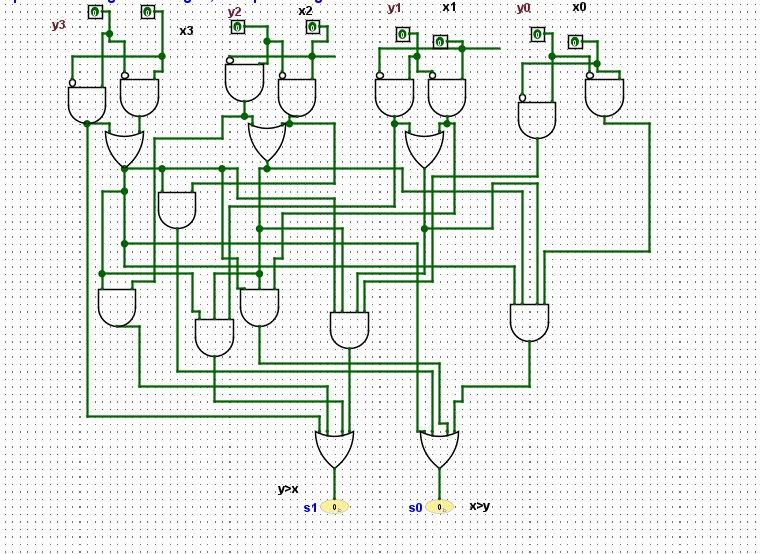
\includegraphics{4bc.jpg}
		\end{figure}
	\end{solution}
	\item Show how five 4-bit comparators can be cascaded to compare two 16-bit
	numbers.	
\end{enumerate}


\end{questions}



\end{document}